\chapter{Introduction}
\label{cap:introduction}

\section{The Company}
\href{https://www.221e.com/about-us}{221e S.r.l.}\footcite{site:221e}, an innovative startup established in 2012 in Italy, has business units in Padova, Treviso, and Bergamo. The company leverages advancements in IT, microelectronics, sensors, and control algorithms to develop miniaturized wireless embedded systems.

Operating under a dual-layer business model, 221e offers:
\begin{enumerate}
    \item OEM (Original Equipment Manufacturer) services to third-party clients needing a technology partner for product development. This involves R\&D contracts followed by commercial agreements for the supply of engineered systems or technology licensing.
    \item Finished products, particularly general-purpose multi-sensor hardware platforms, to direct customers or distributors.
\end{enumerate}

Targeting the Wearable Devices market and the broader Internet of Things (IoT) industry, 221e capitalizes on the limitless applications within these fields. The name 221e, which represents the infinity Unicode character (\(\infty\)), reflects this boundless potential.

Despite being a small business, 221e is rapidly growing, driven by innovation and entrepreneurship, riding the wave of IoT and wearable device advancements.

\begin{figure}[htbp]
    \centering
    
\includegraphics[height=2cm]{221e_logo.png}
    \caption{221e's logo}
\end{figure}

\begin{figure}[htbp]
    \centering
    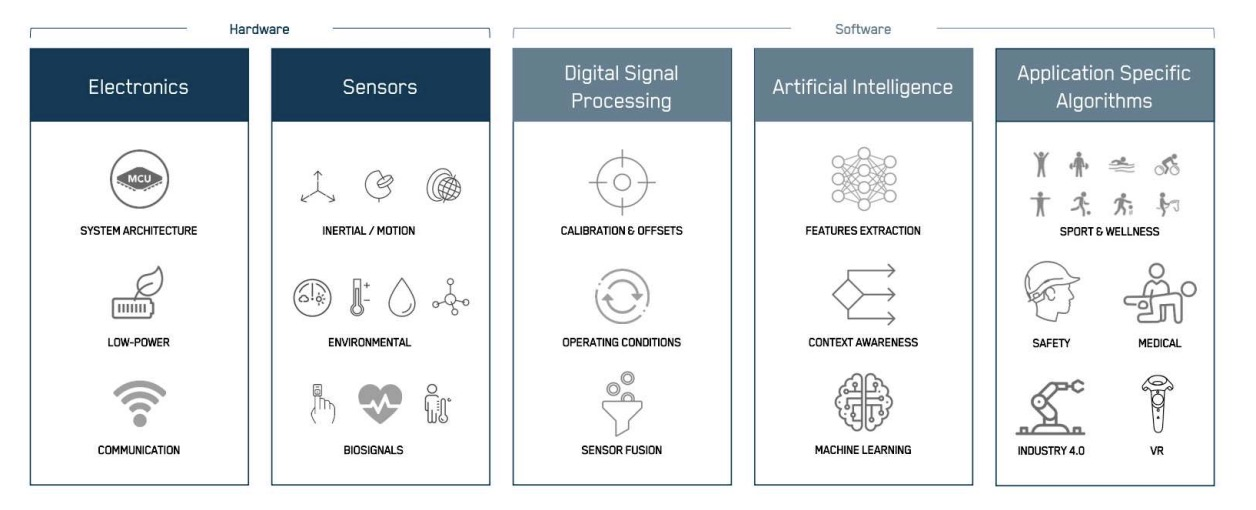
\includegraphics[width=\textwidth]{221e_applications.png}
    \caption{221e's technology echosystem}
\end{figure}


\newpage
\section{Objectives and requirements}

The idea behind the project is to create a cloud-agnostic architecture for the 221e's IoT devices. The architecture should be able to ingest data from multiple sources, store it and  analyze it. The architecture should be able to scale horizontally and vertically, and should be able to be deployed on multiple cloud providers.

\subsection{Cloud Infrastructure}
The system must be able to ingest, store and process large amount of IoT data leveraging the power of any cloud provider present in the market. The final product to be developed is a cloud agnostic architecture that can be deployed on any cloud provider. The main advantage of a cloud agnostic architecture is that it can be deployed on any cloud provider, virtually without any modification. This allows customers to choose the cloud provider that best fits his needs.
The providers taken into account to develop the architecture during this project are the following: \href{https://www.arubacloud.com/}{Aruba Cloud}\footcite{site:aruba-cloud}, \href{https://aws.amazon.com/it/}{Amazon Web Services}\footcite{site:aws} and \href{https://azure.microsoft.com/it-it/}{Microsoft Azure}\footcite{site:azure}. 
AWS and Azure were chosen because the already developed experience by the company and me while Aruba Cloud was chosen because of a partnership between the company and the cloud provider that started during the development of the project.\\


\subsection{Data collection}
The system must be able to ingest data from online devices and on-premise data sources. 
Online devices are devices that are connected to the internet and can send data to the cloud via MQTT protocol.
On-premise data source are offline files that are stored on a local machine and must be uploaded to the cloud. The system must provide a way to upload these files to the cloud.
\subsection{Data processing}
The system must be able to preprocess the data before storage. The preprocessing of the data includes data validation, data cleaning and data transformation, this can be done in cloud or on-premise. The system must be also able to process data after storage. The processing of the data includes data analysis and machine learning operations. The goal of the data processing is to extract useful information from the data and to provide insights to the customer.\\ 

\subsection{Security}
Security is a major concern for the system. In certain scenarios, the data collected could be sensitive and thus must be protected both in transit and at rest.
    \subsubsection{Security in transit}
    Data in transit are transfered using MQTT protocol which is not encrypted by default. The system must provide a way to encrypt and secure the data in transit. MQTT brokers however supports authentication and authorization through certificates as well as TLS/SSL encryption. Using a broker that supports these features is a must.
    
    \subsubsection{Security at rest}
    Data at rest is stored in cloud storage. The cloud storage must provide a way to encrypt the data at rest. The system must also provide a way to manage the encryption keys. Each cloud service provider taken into account provide a way to encrypt data at rest and manage the encryption keys.\\ 
    Furthermore, each cloud provider uses a shared responsibility model for security.
    
    \newpage
    \textbf{Aruba Shared Responsibility Model}
    \href{https://kb.arubacloud.com/en/computing/use-and-technology/shared-responsibility-model.aspx}{Aruba Shared Responsibility Model}\footcite{site:aruba-shared-responsibility-model} is a model that defines the responsibilities of Aruba and the customer for security. Aruba is responsible for the security of the cloud, while the customer is responsible for security in the cloud.\\ The responsibilities of the customer and Aruba varies depending on the service, as shown in the following table.\\ 
    \begin{figure}[htbp]
        \centering
        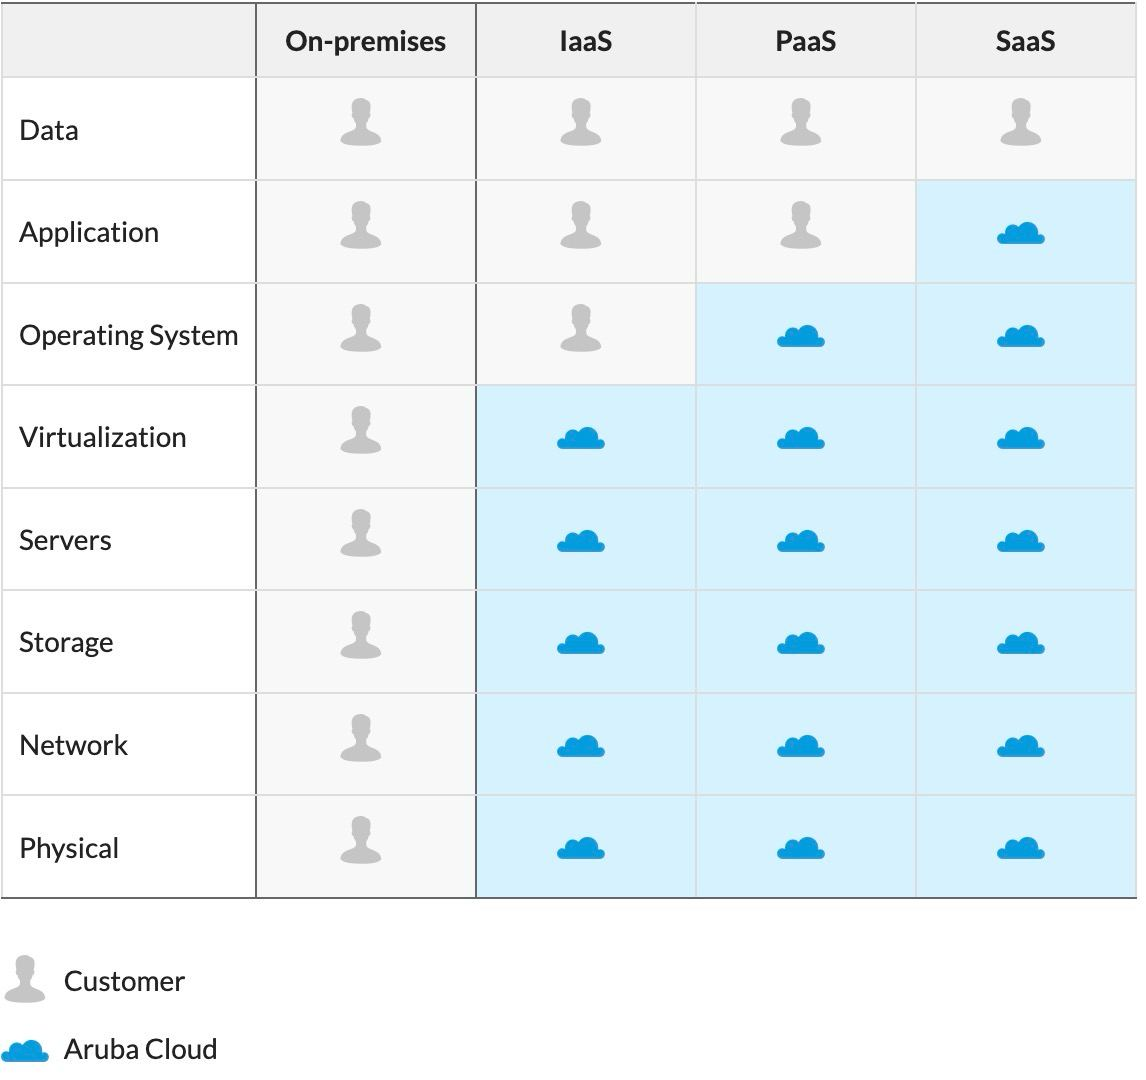
\includegraphics[width=1\textwidth]{aruba-shared-responsibility-model.png}
        \caption{Aruba Shared Responsibility Model}
    \end{figure}

    \newpage
    \textbf{AWS Shared Responsibility Model}
    \href{https://aws.amazon.com/it/compliance/shared-responsibility-model/}{AWS Shared Responsibility Model}\footcite{site:aws-shared-responsibility-model} is a model that defines the responsibilities of AWS and the customer for security. AWS is responsible for the security of the cloud, while the customer is responsible for security in the cloud.\\
    It's important to keep in mind that services in services catalogued as \textit{Infrastructure as a Service} (IaaS) the customer is responsible for the security of the operating system and the applications, while in fully managed services the customer is responsible only for the security of the data.\\
    \begin{figure}[htbp]
        \centering
        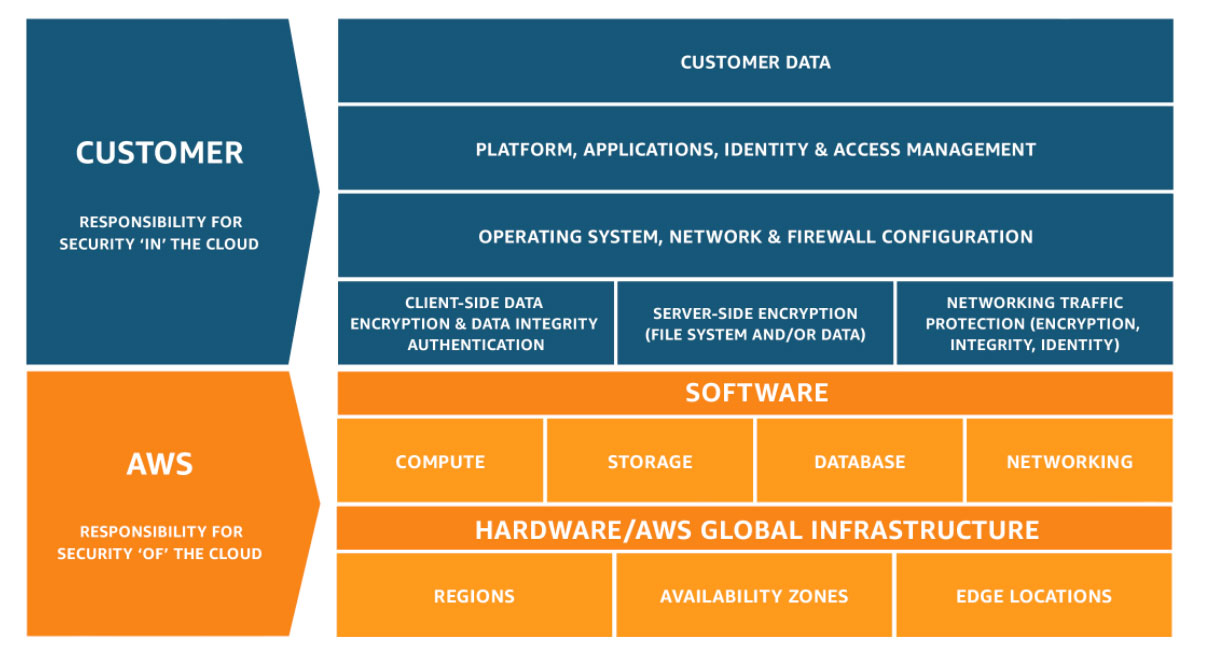
\includegraphics[width=1\textwidth]{aws-shared-responsibility.png}
        \caption{AWS Shared Responsibility Model}
    \end{figure}

    \newpage
    \textbf{Azure Shared Responsibility Model}
    \href{https://learn.microsoft.com/en-us/azure/security/fundamentals/shared-responsibility}{Azure Shared Responsibility Model}\footcite{site:azure-shared-responsibility-model} is a model that defines the responsibilities of Microsoft and the customer for security. The responsibility varies depending on wheter the service is \textit{Software as a Service} (SaaS), \textit{Platform as a Service} (PaaS), \textit{Infrastructure as a Service} (IaaS) or on premise. Regardless of the deployment type, the customer always detain data, endpoints account and access management responsibilities.\\
    
    \begin{figure}[htbp]
        \centering
        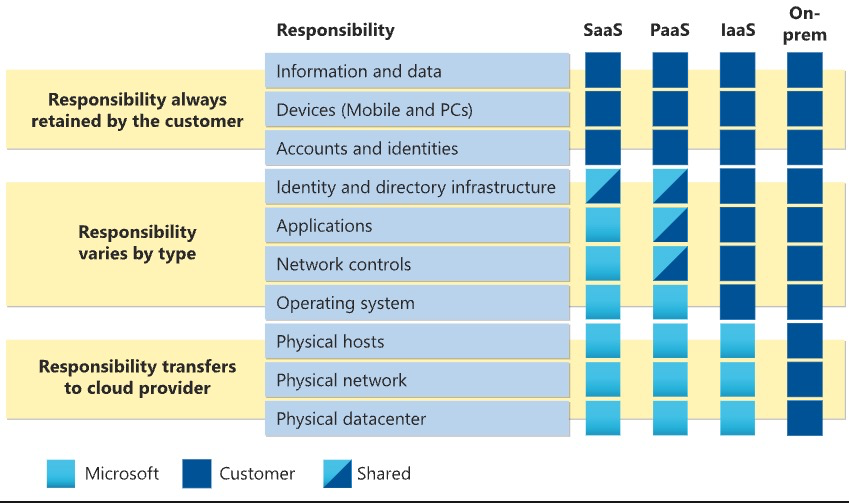
\includegraphics[width=1\textwidth]{azure-shared-responsibility.png}
        \caption{Azure Shared Responsibility Model}
    \end{figure}

\subsection{Scalability}
The system must be able to scale horizontally by adding more instances of the same service and must be able to scale vertically by increasing the resources of the service. The system must be able to automatically scale based on the load of the system.
Stress tests must be performed to verify the scalability of the system.\\

